\chapter{EXPERIMENTACIÓN Y EVALUACIÓN}

\section{Pruebas}

\section{Matriz de confusión}

\noindent La matriz de confusión es una herramienta que permite la visualización del desempeño del modelo clasificador empleado en el aprendizaje supervisado. Para este caso en particular se tienen dos modelos y cada uno de estos modelos tendrá su matriz de confusión. En la figura \sout{acá poner la dirección de la figura} cada columna de la matriz representa el número de predicciones de cada clase, mientras que cada fila representa a las instancias en la clase real.

\begin{figure}[H]
\centering
{\includegraphics[width=1\textwidth , frame]{imagenes/1matrizconfusion.png}}
%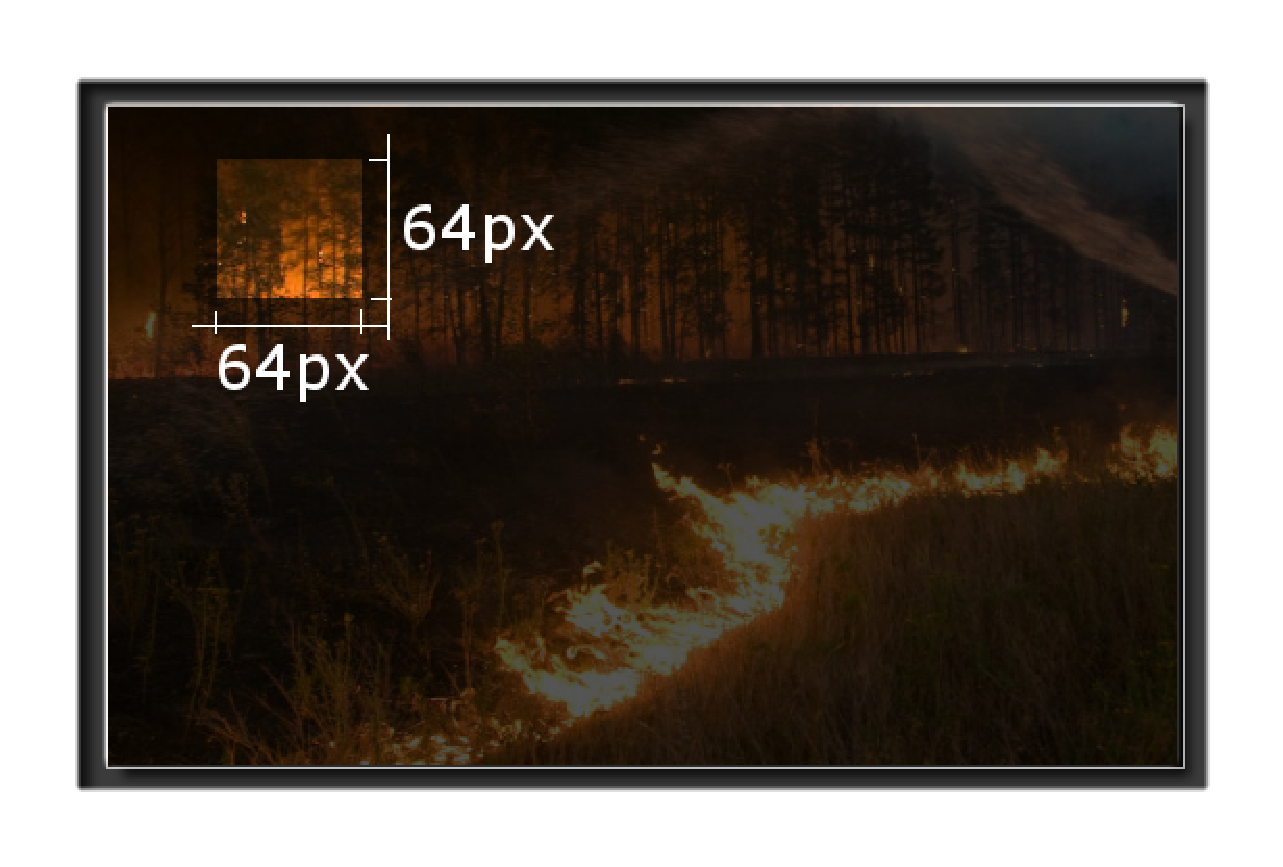
\includegraphics[width=0.5\textwidth , frame]{./imagenes/tratamiento/recorte}
\caption{Sección de la imagen que sera recortada.}
\label{fig:sectorRecorte}
\end{figure}

Las instancias de cada clase real son las muestras positivas y negativas del conjunto de validación. En base a estos datos:
\begin{itemize}
\item[1. ] El cuadro \textbf{verdaderos positivos} representa la cantidad de muestras positivas que fueron detectadas como positivas.
\item[2. ] El cuadro \textbf{falsos positivos} representa la cantidad de muestras negativas que fueron detectadas como positivas.
\item[3. ] El cuadro \textbf{falsos negativos} representa la cantidad de muestras positivas que fueron detectadas como negativas.
\item[4. ] El cuadro \textbf{verdaderos negativos} representa la cantidad de muestras positivas que fueron detectadas como negativas.
\end{itemize}

\noindent Estos datos permiten obtener diferentes tipos de datos tales como la precisión, exactitud y la sensibilidad del modelo clasificador.

\section{Rendimiento del clasificador}

\noindent Para evaluar el rendimiento del modelo clasificador, utilizamos el conjunto de validación generado durante el proceso de generación del modelo clasificador.

\subsection{Exactitud}

\noindent La exactitud es la proximidad del resultado con la clasificación exacta y se representa mediante la siguiente formula:

\begin{center}
\begin{math}
Exactitud = \frac{\# RealesPositivos + \# RealesNegativos}{\# TotalDePredicciones}
\end{math}
\end{center}

\paragraph{Modelo clasificador de fuego:} \sout{100\%} de exactitud.

\paragraph{Modelo clasificador de humo:} \sout{100\%} de exactitud.

\subsection{Precisión}

\noindent La precisión es la calidad del resultado positivo del clasificador:

\begin{center}
\begin{math}
Exactitud = \frac{\# RealesPositivos}{\# RealesPositivos + \# FalsosPositivos}
\end{math}
\end{center}

\paragraph{Modelo clasificador de fuego:} \sout{100\%} de precisión.

\paragraph{Modelo clasificador de humo:} \sout{100\%} de precisión.

\subsection{Tasa de detección}

\noindent O Sensibilidad, es la eficiencia en la clasificación de todos los elementos que son de la clase.

\begin{center}
\begin{math}
Exactitud = \frac{\# RealesPositivos}{\# RealesPositivos + \# FalsosNegativos}
\end{math}
\end{center}

\paragraph{Modelo clasificador de fuego:} Tasa de detección de \sout{100\%}.

\paragraph{Modelo clasificador de humo:} Tasa de detección de \sout{100\%}.

\subsection{Especificidad}

\noindent Es la eficiencia en la clasificación de todos los elementos que no son de la clase.

\begin{center}
\begin{math}
Exactitud = \frac{\# Reales Negativos}{\# Reales Negativos + \# Falsos Positivos}
\end{math}
\end{center}

\noindent La especificidad permite encontrar la Tasa de error del modelo clasificador mediante la siguiente formula:

\begin{center}
\begin{math}
Tasa De Error = 1 - Especificidad
\end{math}
\end{center}
\paragraph{Modelo clasificador de fuego:} Tasa de error de \sout{100\% }.

\paragraph{Modelo clasificador de humo:} Tasa de error de \sout{100\% }.

\noindent Estos resultados serán analizados en el siguiente capitulo.

\section{Evaluación del sistema de detección}

\subsection{Tasa de detección}

\subsection{Tasa de Error}

\subsection{Falsos positivos por imagen}

\section{Casos de estudio}